\documentclass{article}
\usepackage{graphicx} % Required for inserting images
\usepackage[margin=1in]{geometry}
\usepackage{amsmath}
\usepackage{amsthm}
\usepackage{amssymb}
\usepackage{amsfonts}
\usepackage{enumitem}
\usepackage{verbatim}
\usepackage{xcolor}
\usepackage{soul}

\title{Homework 3: Report}
\author{Dante Buhl}

\DeclareMathOperator{\cond}{cond}
\DeclareMathOperator{\vecspan}{span}

\begin{document}

\newcommand{\bs}[1]{\boldsymbol{#1}}
\newcommand{\bmp}[1]{\begin{minipage}{#1\textwidth}}
\newcommand{\emp}{\end{minipage}}
\newcommand{\R}{\mathbb{R}}
%\newcommand{\Imag}{\mathbb{I}}
\newcommand{\C}{\mathbb{C}}
\newcommand{\N}{\mathcal{N}}
\newcommand{\I}{\mathrm{I}}
\newcommand{\K}{\bs{\mathrm{K}}}
\newcommand{\m}{\bs{\mu}_*}
\newcommand{\s}{\bs{\Sigma}_*}
\newcommand{\dt}{\Delta t}
\newcommand{\tr}[1]{\text{Tr}(#1)}
\newcommand{\Tr}[1]{\text{Tr}(#1)}

\maketitle

\section*{Question 1: BVP for 2D Poisson's Equation}
\begin{enumerate}[label=\alph*)]

    \item Write Code to solve (1)
    \begin{align}
        \begin{cases}
            \nabla^2 U(x,y) = f(x,y) \quad &(x, y) \in \Omega\\
            U(x,y) = g(x,y) \quad &(x,y) \in \partial\Omega,\\
            f(x,y) = -20 +3x^2 + 4y^2\\
            g(x,y) = 2 - x^2 + 2\sin(\pi y^2)
        \end{cases} 
    \end{align}

    \item 
    \begin{figure}[ht]
        \centering
        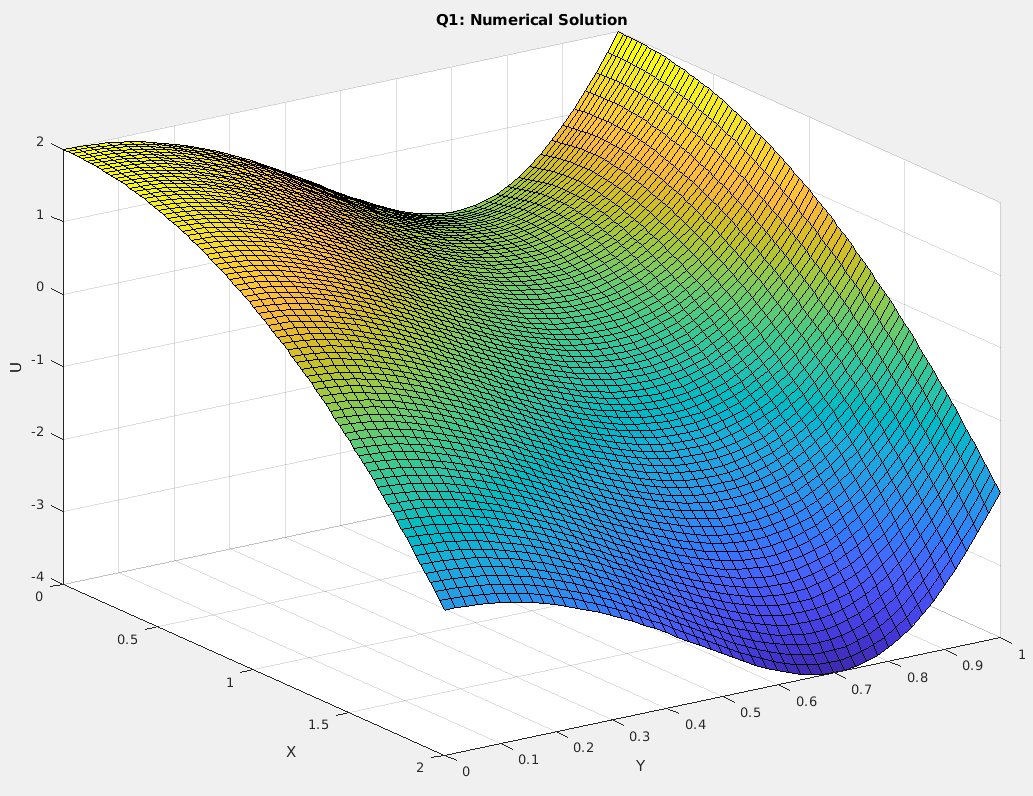
\includegraphics[width=.6\textwidth]{q1_num_sol.png}
        \caption{Numerical Solution to (1) with $N=81, M=51$}
    \end{figure}

    \item 
    \begin{figure}[ht]
        \centering
        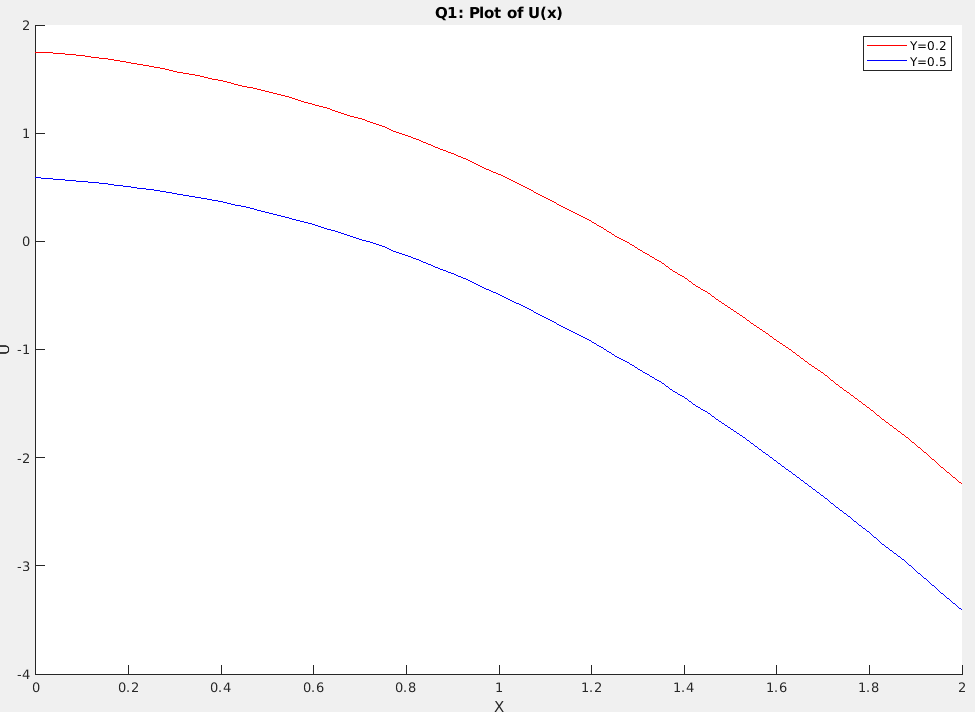
\includegraphics[width=.6\textwidth]{q1_num_sol_yconst.png}
        \caption{Numerical Solution to (1) at $Y=0.2, 0.5$}
    \end{figure}

\end{enumerate}


\section*{Question 2: IBVP for 1D Heat Equation}

\begin{enumerate}[label=\alph*)]

    \item Determine the analytical solution for (2)
    \begin{align}
        \begin{cases}
            U_t = U_{xx}\quad \quad x \in [-1, 1],
            \quad t \ge 0\\
            U(x,0) = (3+x) + 5(1 - x^2)^2\\
            U(-1,t) = 2, \quad U(1, t) = 4
        \end{cases} 
    \end{align}
    \[
        g(x) =  3 + x + 5 - 10x^2 + 5x^4
    \]
    \begin{proof}
        To begin we look at the general solution for the Heat Equation with
        Homogeneous BC.
        \begin{align*}
            \begin{cases}
                \eta = U - g(x) = U - (3+x) + 5(1 - x^2)^2\\
                \eta_t = \eta_{xx} - 20 + 60x^2 \quad \quad x \in [-1, 1],
                \quad t \ge 0\\
                \eta(x,0) = 0\\
                \eta(-1,t) = 0, \quad \eta(1, t) = 0
            \end{cases}
        \end{align*}
        
    \end{proof}
    \item \hl{Plot the analytical solution as a surface plot over [x, t]}

    \item \hl{Write code and integrate using second-order finite differences and CN}

    \item \hl{Wrote code and integrate using Gauss-Chebyshev-Lobatto coallocation
    method}

    \item \hl{plot maximum pointwise error on a log scale plot between analytical
    and numerical solutions}

\end{enumerate}

\section*{Question 3: Extra Credit}

\begin{enumerate}[label=\alph*)]

    \item \hl{Write code to compute the nuemrical solution using secondorder finite
    diff, and AB2.} 

    \item \hl{plot the numerical solution as a surface plot}

    \item \hl{plot the numerical sollution at t = 62 as a function of x.}

\end{enumerate}

\end{document}
